% Figure s03f02_bulkboundary (Session 3): the bulk-boundary correspondence as an argument about an integer.
% The image is rendered by figures/blender/s03f02_bulkboundary.py; the coordinates of the labels come from
% figures/blender/out/s03f02_bulkboundary_anchors.tex. Build with figures/blender/build_figure.sh s03f02_bulkboundary.
\documentclass[11pt,tikz,border=0pt]{standalone}
\usepackage[T1]{fontenc}
\usepackage{amsmath,amssymb,graphicx,bm}
\usepackage{xcolor}
\usetikzlibrary{arrows.meta,calc}
% The three label colors of the figures, with the same values as in src/figures_preamble.tex.
\definecolor{aqmaccent}{RGB}{31,78,121}
\definecolor{aqmbroken}{RGB}{168,42,34}
\definecolor{aqmmuted}{RGB}{125,125,125}

\newlength{\figw}\setlength{\figw}{14.78cm}   % 0.81 of the text width, before the empty margins of the render are cropped

\begin{document}
\begin{tikzpicture}[lbl/.style={font=\small, inner sep=1.5pt}, pnl/.style={font=\small\bfseries, inner sep=1.5pt}]
  \node[overlay, anchor=south west, inner sep=0pt] at (0,0)
    {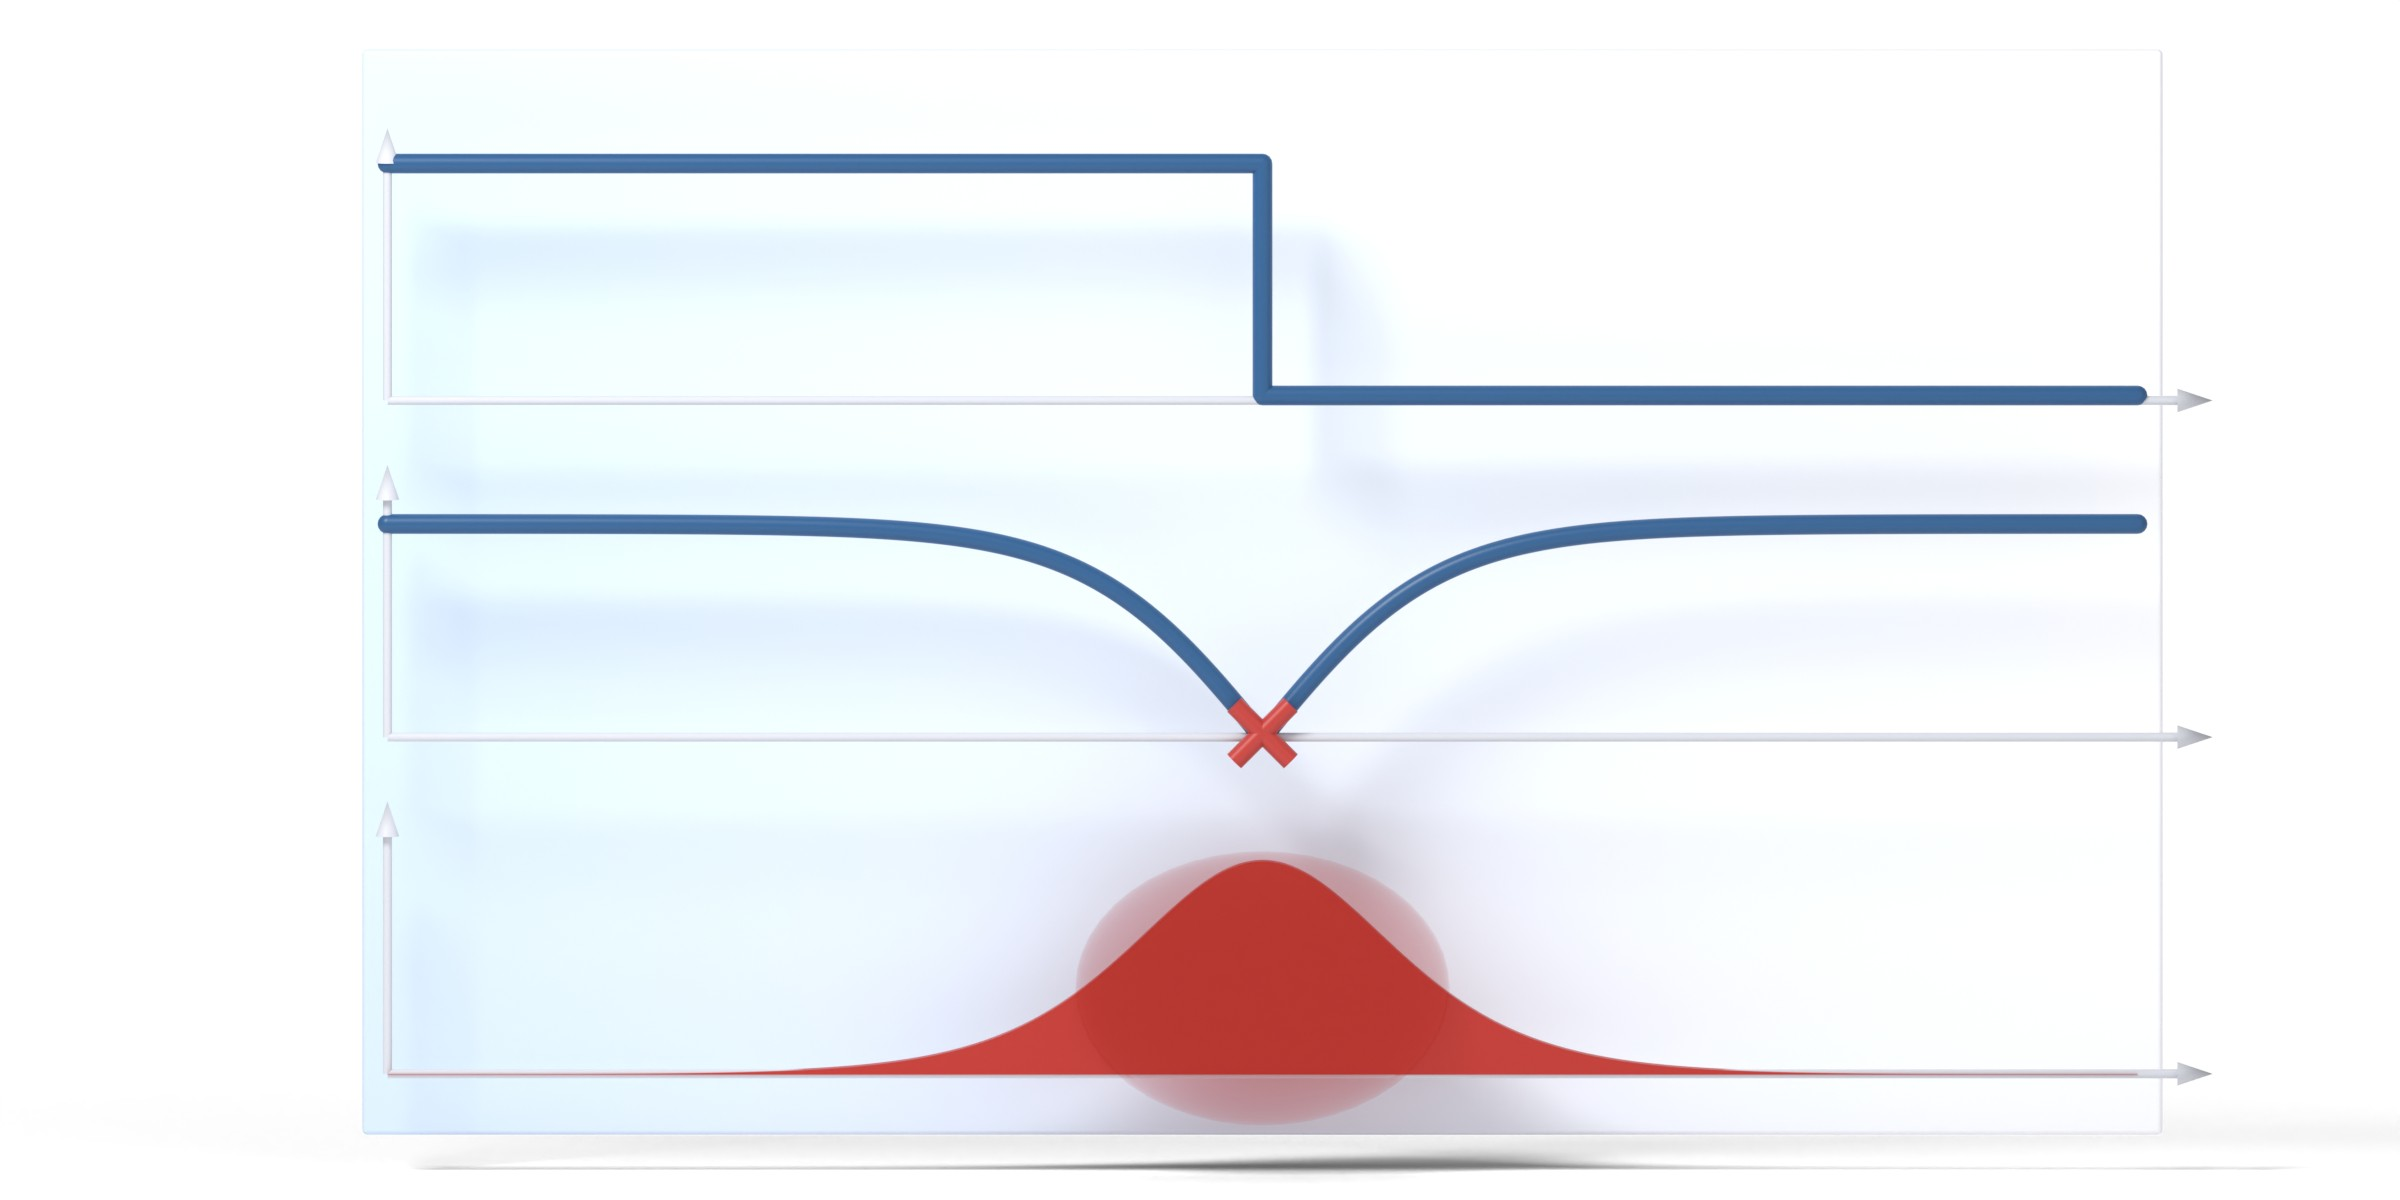
\includegraphics[width=\figw]{../blender/out/s03f02_bulkboundary.jpg}};
  % written by build_figure.sh; the painted part of the image
\path (0.1508\figw,0.0079\figw) rectangle (0.9988\figw,0.4796\figw);

  %% written by figlib.py; x and y in units of the image width
\coordinate (C1) at (0.3438\figw,0.4370\figw);
\coordinate (C2) at (0.7083\figw,0.3435\figw);
\coordinate (Clab) at (0.1510\figw,0.3825\figw);
\coordinate (glab) at (0.1510\figw,0.2422\figw);
\coordinate (plab) at (0.1510\figw,0.1019\figw);
\coordinate (H1) at (0.1771\figw,0.4682\figw);
\coordinate (H2) at (0.8750\figw,0.4682\figw);
\coordinate (x) at (0.9219\figw,0.0526\figw);

  \node[lbl, anchor=south] at (C1) {$C_1=1$};
  \node[lbl, anchor=south] at (C2) {$C_2=0$};
  \node[lbl, anchor=east, align=right] at (Clab) {Chern\\number};
  \node[lbl, anchor=east, align=right] at (glab) {local\\gap};
  \node[lbl, anchor=east, align=right, text=aqmbroken] at (plab) {bound\\state};
  \node[lbl, anchor=north west] at (H1) {$H_1$};
  \node[lbl, anchor=north east] at (H2) {$H_2$};
  \node[lbl, anchor=south east] at (x) {$x$};
\end{tikzpicture}
\end{document}
